\subsection{\acs{ENISA} - Good Practice Guide for Incident Management}
This guide is developed by the \ac{ENISA} and provides a description of good practices for security incident management. The content is, unless specified otherwise, derived from \cite{enisaGuide}. The focus of this guide is IT and information security incidents. It specifically addresses the incident handling part of incident management. The incident management and incident handling processes are illustrated in figure \ref{fig:ENISAIncidentManagement}. The incident handling process has four major components, as shown in the figure. 

\begin{figure}[h]
\begin{center}
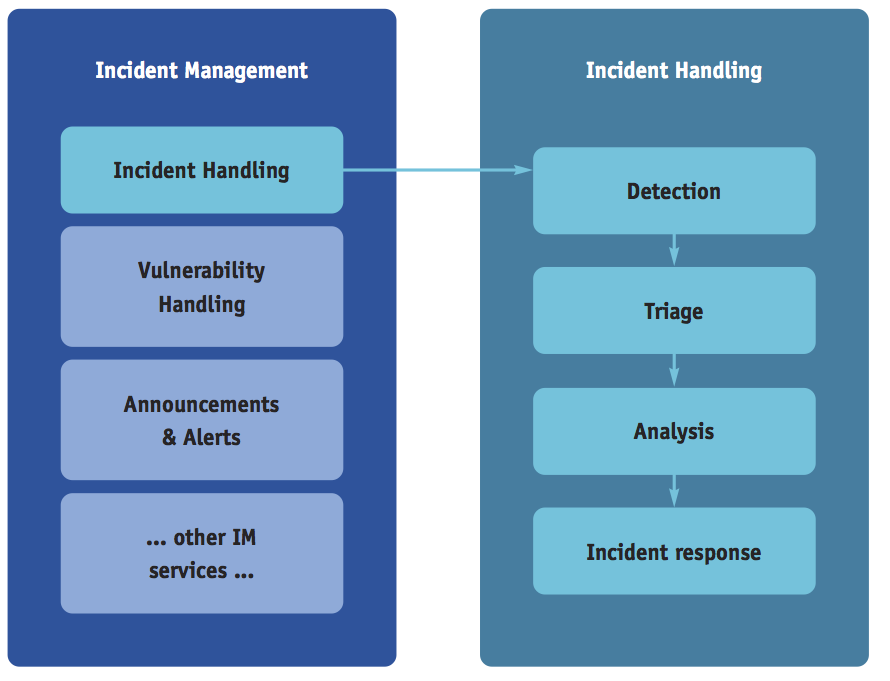
\includegraphics[scale=0.74]{enisaIncidentManagement.png}
\caption[ENISA Incident Management and Incident Handling]{Incident Management and Incident Handling \cite{enisaGuide}}
\label{fig:ENISAIncidentManagement}
\end{center}
\end{figure}

\paragraph{Detection:} The \ac{CERT} can receive incident reports from various sources. This guide recommends to use e-mail as a communication channel as people prefer this. Additionally, it recommends to use monitoring systems in addition to reports sent by others. Detection includes registration of incident reports in an incident handling system. This stage is a good place to implement pre-filtering mechanism for incident reports. The registration process could include the use of an incident report form.

\paragraph{Triage:} This stage consists of the three phases verification, initial classification and assignment. During these phases the following questions should be answered:

\begin{itemize}\itemsep-0.2cm
\item Is it really an IT security incident?
%\item Is it related to one of your constituents?
%\item Does it fit within the mandate the \ac{CERT} has?
\item What is the impact?
\item Is there collateral damage?
%\item How fast could it spread to other constituents?
\item How many people do you need to handle this incident?
\item Which incident handler should be appointed to the incident?
\end{itemize}

The verification phase seeks to answer the first question. It is however recommended to respond to and archive all reports, even those not defined as information security incidents. They may include information relevant to other incidents or potentially lead to an incident. After an incident report has been verified the incident should be initially classified according to a classification schema. The last part of the triage component is to assign the incident to an incident handler.

\paragraph{Analysis and Incident response:} These components are illustrated by figure \ref{fig:IncidentResolutionCycle}. The cycle may need to be iterated several times. To perform \textit{data analysis} there should be collected as much data as possible. Prior to the collection, all involved parties should be notified. Sources for data collection could be an incident reporter, monitoring systems, a referring database and relevant log files. The collected data should be used to try to determine the source of the incident. Prior to the data analysis, decisions about what data to analyse and in what order must be made. During the analysis, people will often exchange ideas and observations as well as draw conclusions. This belongs to the \textit{resolution research}. It is recommended to advise team members to write down any observations that can be discussed in review meetings. The \textit{action proposed} part consists of preparing a set of tasks for each party involved. The \textit{action performed} should be monitored, where possible. The main goal for all actions is the \textit{eradication and recovery}.

\begin{figure}[h]
\begin{center}
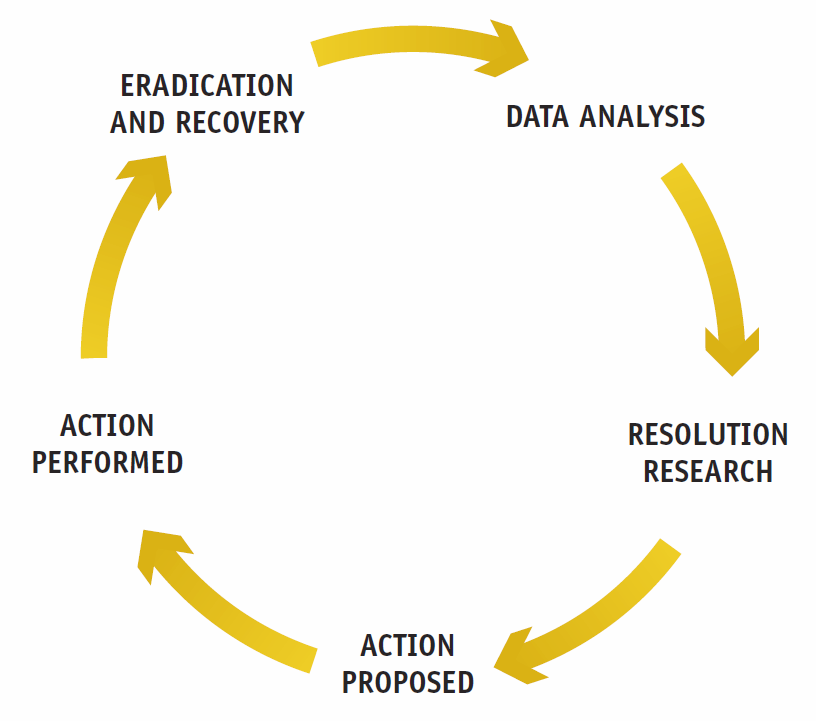
\includegraphics[scale=0.4]{IncidentResolutionCycle.png}
\caption[ENISA Incident Resolution Cycle]{Incident Resolution Cycle \cite{enisaGuide}}
\label{fig:IncidentResolutionCycle}
\end{center}
\end{figure}

When you have left the incident resolution cycle, there are still tasks to perform. The incident needs to be closed properly. Each involved party needs to be informed that the incident is resolved. The classification of the incident should be revisited and a final classification should be performed. The classification could have been revisited during the resolution cycle as well. It is recommended to have a taxonomy and to classify incidents in accordance with it.

After an incident has been resolved or closed a post-analysis should be performed in order to learn from the incident. It is also recommended not to analyse all incidents, but only the most characteristic and complex ones and those that include new attack vectors. 

Incidents should be reported to the management. In addition to specific issues, the daily operations should be reported, including costs, positive results, plans and risks. This will save time and resources in situations where you need the management's operational or financial support and quick decisions.



